\subsection{Diskrete Signale}

Wir sind nun endlich im Digitalen angekommen. 
Wir wollen uns als erstes verschiedene M"oglichkeiten der Klassifikation von diskreten Signalen $x[\cdot] : \Z \rightarrow \C$ ansehen.
Dabei folgend wir weitestgehend~\cite[Kap.~2.1]{proakis2013}.
In \cref{sec:spec_sig} haben wir bereits den Einheitssto"s $\delta[\cdot]$ und die Heavy-Side-Funktion $u[\cdot]$ kennengelernt.

\begin{itemize}
    \item Eine linear ansteigende Version $u_r[\cdot]$ von $u[\cdot]$ ist gegeben durch
    \[
        u_r[n] = n \cdot u[n] = \begin{cases}
            n, \Text{f"ur} n \geqslant 0 \\
            0, \Text{sonst}.
        \end{cases}
    \]
    In Python ist die Funktion auch sehr einfach zu implementieren:
\begin{minted}{python3}
def u_r(n: int) -> int:
    return n if n>0 else 0
\end{minted}
Will man die Funktion effizienter mittels Numpy~\cite{numpy} implementieren, dann liest sie sich
\begin{minted}{python3}
import numpy as np
def u_r_np(n: np.ndarray[int]) -> np.ndarray[int]:
    u_r = n.copy()
    u_r[n <= 0] = 0
    return u_r
\end{minted}
\item F"ur eine komplexe Zahl $a = r \exp(\jmath \theta) \in \C$ erh"alt man das zugeh"orige exponentielle Signal als
\[
    x[n] 
        = a ^ n 
        = r^n \exp(\jmath \theta n) 
        = r^n \cos(\theta n) + \jmath r^n \sin(\theta n).
\]
Damit gilt $x[0] = 1$ unabh"angig von $a$.
Beispielsweise erhalten wir das Signal $x_k$ aus \eqref{eq:disc_harms_comp} indem wir $r=1$ und $\theta = 2 \pi k f_0$ setzen.
Eine Implementierung von $x[n]$ is in \Cref{py:complex_exp} gegeben.
Es ist sicher interessant f"ur verschiedene Werte von $a$ und $\bm n$ die Ausgabe zu betrachten.

Beispielsweise kann man sehen, dass f"ur $a \in \R$ gelten muss, dass $\lim_{n \rightarrow \infty} x[n] = 0$, falls $a < 0$, aber $\lim_{n \rightarrow -\infty} \Abs{x[n]} = \infty$ andernfalls.
Weiterhin gilt f"ur $a \in \C$ und $\Abs{a} = 1$, dass dann auch $\Abs{x[n]} = 1$ f"ur alle $n$.
\end{itemize}
%
\begin{listing}
    \noindent
    \begin{minipage}{0.49\textwidth}
        \strut\vspace*{-\baselineskip}\newline
        \inputminted[firstline=4]{python3}{code/complex_exp.py}
    \end{minipage}%
    \begin{minipage}{0.49\textwidth}
        \strut\vspace*{-\baselineskip}\newline
        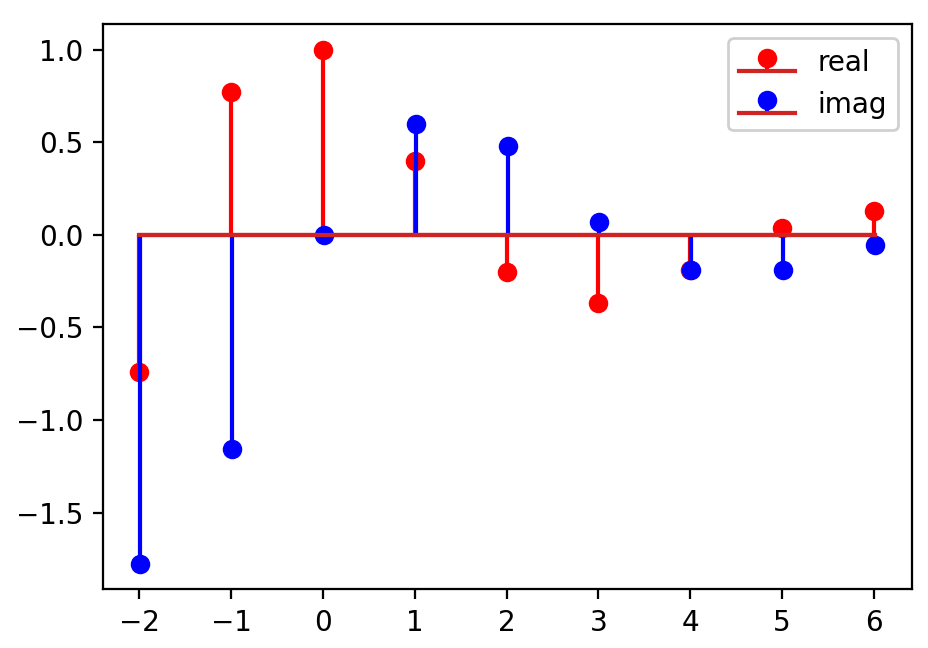
\includegraphics[width=\textwidth]{code/complex_exp.png}
    \end{minipage}
    \codecaption{code/complex_exp.py}{Berechnung und Darstellung eines komplexen exponentiellen Signals}\label{py:complex_exp}
\end{listing}
%
\subsubsection{Energie Diskreter Signale}

Oft ist es interessant zu bemessen, wie viel Energie in einem Signal vorhanden ist.
F"ur eine physikalisch korrekte Bemessung dieser Energie, m"usste man das Signal zwar mit Einheiten versehen, aber diese ergeben nur einen entsprechenden Proportionalit"atsfaktor.
Hierzu betrachten wir
\begin{equation}\label{eq:disc_sig_energy}
    E(x[\cdot]) 
        = \Sum{n \in \Z}{}{\Abs{x[n]}^2} 
        = \Sum{n \in \Z}{}{x[n]^\ast \cdot x[n]}.
\end{equation}
Wenn gilt $E(x[\cdot]) < \infty$, dann sprechen wir erstaunlicherweise von einem Signal endlicher Energie.

Es ist nun interessant sich eine Menge $\mathcal{E}$ zu definieren, die alle Signale enth"alt, welche endliche Energie besitzen, also 
\[
    \mathcal{E} = \{x : \Z \rightarrow \C \Text{mit} E(x[\cdot]) < \infty\}.
\]
Man kann sich nun "uberlegen, dass
\[
E(\alpha x[\cdot] + \beta y[\cdot]) 
    \leqslant E(\alpha x[\cdot]) + E(\beta y[\cdot])
    = \alpha^2 E(x[\cdot]) + \beta^2 E(y[\cdot]) 
    < \infty 
\]
gelten muss, falls $E(x[\cdot]),E(y[\cdot]) < \infty$. 
Das hei"st, dass Linearkombinationen von Signalen mit endlicher Energie wieder ein Signal mit endlicher Energie ergeben.
Das hei"st, dass die Signale endlicher Energie bilden einen \emph{Unterraum}.
Wir k"onnen noch einen Schritt weiter gehen und wie in \eqref{eq:dtft_inner_prod} die Summe in \eqref{eq:disc_sig_energy} als Skalarprodukt auffassen.

Definieren wir f"ur zwei Signale endlicher Energie die Abbildung $\ScPr{\cdot}{\cdot} : \mathcal{E} \times \mathcal{E} \rightarrow \C$ als
\begin{equation}\label{eq:disc_inner_prod}
    (x[\cdot], y[\cdot]) 
        \mapsto \ScPr{x[\cdot]}{y[\cdot]}
        = \Sum{n \in \Z}{}{x[n]^\ast \cdot y[n]},
\end{equation}
dann kann man sich "uberlegen, dass dies die Bedingungen an ein \emph{Skalarprodukt} erf"ullt.
Beispielsweise kann man nachrechnen, dass die unendliche Summe in \eqref{eq:disc_inner_prod} immer endlich ist, falls $x[\cdot], y[\cdot] \in \mathcal{E}$, da
\[
\Abs{\ScPr{x[\cdot]}{y[\cdot]}} \leqslant E(x[\cdot]) \cdot E(y[\cdot]) < \infty
\]
Nun kann man aber auch $E$ durch
\[
E(x[\cdot]) = \ScPr{x[\cdot]}{x[\cdot]}
\] 
ausdr"ucken.

\begin{Bsp}
Betrachten wir $x[n] = a^n \cdot u[n]$ f"ur $a = r \exp{\jmath \theta} \in \C$.
Dann berechnet sich $E(x[\cdot])$ durch
\[
E(x[\cdot]) 
    = \Sum{n \geqslant 0}{}{\Abs{a^n}^2} 
    = \Sum{n \geqslant 0}{}{\left(r^2\right)^n}.
\]
Ist nun $r \geqslant 1$, dann $E(x[\cdot]) = \infty$, falls aber $r < 1$, dann ergibt sich aus der geometrischen Reihe, dass
\[
    E(x[\cdot]) = \frac{1}{1 - r^2}
\]
gilt.
Das hei"st auch, dass das Heavy-Side-Signal $u[\cdot]$ keine endliche Energie besitzt.
\end{Bsp}
%
\subsubsection{Periodische Signale}
%
Gilt f\"ur ein Signal $x[\cdot]$, dass $x[n + N] = x[n]$ f"ur ein $N \in \N$ und \emph{alle} $n \in \Z$, so nennt man $x[\cdot]$ periodisch mit Periodenl"ange/Periode $N$, oder kurz $N$-periodisch, siehe beispielsweise \Cref{eq:disc_harms_comp}.
Falls $x[\cdot]$ nun $N$-periodisch ist, dann ist $x[\cdot]$ auch $kN$-periodisch, falls $k \in \N$.
Das hei"st, dass es sinnvoller ist, das \emph{kleinste} $N \in \N$ zu betrachten, sodass $x[\cdot]$ dann $N$-periodisch ist. 
Man nennt $N$ dann Fundamentalperiode.
Falls solch ein $N$ nicht existiert, dann nennt man $x[\cdot]$ aperiodisch, oder nicht-periodisch.
Falls $x[\cdot] \neq 0$, dann gilt f"ur periodische Signale, dass $E(x[\cdot]) = \infty$.
Beispielsweise haben wir bereits in \Cref{sec:sample_harm} gesehen, dass
\[
x[n] = \exp(\jmath 2 \pi f)
\]
periodisch mit Periode $N$ ist, falls $f = k/N$, also eine rationale Zahl ist.
%
\subsubsection{Symmetrie von Signalen}
%
Gilt f"ur ein Signal $x[n] = x[-n]$, dann nennt man es \emph{symmetrisch} bzw.~\emph{gerade}.
Gilt andererseits $x[n] = -x[-n]$, so nennt man es \emph{anti-symmetrisch} bzw.~\emph{ungerade}.

Ist ein beliebiges Signal $x[\cdot]$ gegeben, so kann man
\[
    x_g[n] = \frac 12 \left(x[n] + x[-n]\right)
    \Text{und}
    x_u[n] = \frac 12 \left(x[n] - x[-n]\right)
\]
definieren.
Dann ist $x_g[\cdot]$ gerade und falls $x[\cdot]$ bereits gerade ist, so gilt $x[\cdot] = x_e[\cdot]$.
Genauso ist $x_u[\cdot]$ ungerade und falls $x[\cdot]$ bereits ungerade ist, so gilt $x[\cdot] = x_u[\cdot]$.
Au"serdem gilt
\[
x[n] = x_g[n] + x_u[n].
\]
Wir haben das Signal $x[\cdot]$ also in einen geraden und einen ungeraden Teil zerlegt.
Dies ist manchmal sinnvoll, wenn man solch ein Signal linear transformiert und wei"s, dass die lineare Transformation f"ur gerade oder ungerade Signale gewisse Eigenschaften hat.
Wie man an \Cref{py:even_odd} gut sehen kann, muss gelten $x_u[0] =0$, da $x_u[0] = x[0] - x[0] = 0$ und $x_e[0] = x[0]$, da $2 x_e[0] = x[0] + x[0]$.
%
\begin{listing}
    \noindent
    \begin{minipage}{0.49\textwidth}
        \strut\vspace*{-\baselineskip}\newline
        \inputminted[firstline=4]{python3}{code/even_odd.py}
    \end{minipage}%
    \begin{minipage}{0.49\textwidth}
        \strut\vspace*{-\baselineskip}\newline
        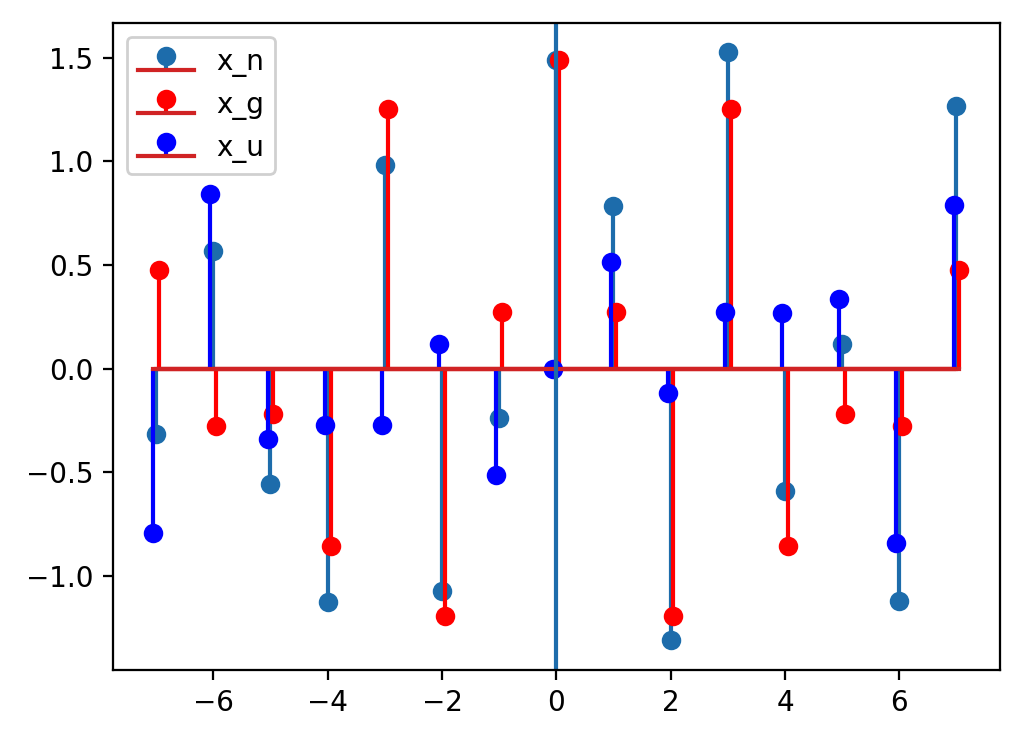
\includegraphics[width=\textwidth]{code/even_odd.png}
    \end{minipage}
    \codecaption{code/even_odd.py}{Zerlegung eines Signals in seinen geraden und ungeraden Anteil.}\label{py:even_odd}
\end{listing}
%
\subsection{Diskrete Systeme}
%
%
Nachdem wir uns nun ein wenig mit diskreten Signalen vertraut gemacht haben, sind wir in der Lage und mit diskreten Systemen zu befassen.
Ganz allgemein kann man fast jeden Prozess, an dessen Anfang ein diskretes Signal steht und dessen Ergebnis wiederum ein diskretes Signal ist, als ein diskretes System auffassen.
Sobald man dieses System nun einmal vorliegen hat, will man Techniken und Werkzeugen entwickeln, wie man dieses System systematisch untersuchen kann -- eine Systematik der Systeme.

Ein System $\mathcal{T}$ wird mathematisch als Abbildung eines (Eingabe-)Signals $x[\cdot]$ auf ein anderes (Ausgabesignal) $y[\cdot]$ aufgefasst. Wir schreiben daf"ur dann
%
\begin{equation}\label{eq:gen_disc_sys}
    x[\cdot] \mapsto \mathcal{T}(x[\cdot])[\cdot] = y[\cdot].
\end{equation}
%
Das System $\mathcal{T}$ bildet also die Paare $(x[\cdot], \mathcal{T}(x[\cdot])) = (x[\cdot], y[\cdot])$.

Betrachten wir folgendes
\begin{Bsp}\label{ex:simple_sys}
    Gegeben sei das Eingabesignal
    \[
    x[n] = \begin{cases}
        \Abs{n}, \Text{falls} -3 \leqslant n \leqslant +3, \\
        0 \Text{sonst.}
    \end{cases}
    \]
    Wir sind nun an den Werten der Ausgabesignals $y[\cdot]$ interessiert, f"ur
    \begin{enumerate}[a)]
        \item das Einheitssystem $y[n] = x[n]$,
        \item das Einheitsdelay-System $y[n] = x[n-1]$,
        \item das Einheitsadvance-System $y[n] = x[n+1]$
    \end{enumerate}
    interessiert.
\end{Bsp}
Diese Systeme waren noch ein wenig simpel und man ist vielleicht noch nicht "uberzeugt, dass eine genauere Analyse von diskreten Systemen notwendig sein sollte.
Dies liegt vor allem daran, dass die Systeme in \Cref{ex:simple_sys} nur \q{lokal} gearbeitet haben, da Werte $y[n]$ nur von Werten $x[n-1]$, $x[n]$ und $x[n+1]$ abh"angen.

Betrachten wir wiederum die Mandelbrot-Iteration, aber diesmal als System
\[
    y[n+1] = y[n]^2 + x[n]
\]
f"ur verschiedene Eingangssignale $x[n] = c \in \C$ mit $y[0] = 0$.
Wir sind nun an solchen $c$ interessiert f"ur welche das System divergiert, also $\Abs{y[n]} > 2$ ab einem gewissen $n$.
Wir wollen aber solche $c$ finden, f"ur welche wir in einem gewissen Bereich $n \in [n_{\rm low}, n_{\rm hgh}]$ divergieren.
Das in \Cref{py:buddhabrot} gezeigte Beispiel ist hierbei am anderen Ende des Komplexit"atsspektrums, da man bei diesem System eher von einem \q{chaotischen} System sprechen sollte. 
Kleine Ver"anderungen an $x[n] = c$ haben gro"sen Einfluss auf das Divergenzverhalten der Folge $y[n]$\footnote{\url{https://erleuchtet.org/2010/07/ridiculously-large-buddhabrot.html}}.
\begin{listing}
    \noindent
    \begin{minipage}{0.49\textwidth}
        \strut\vspace*{-\baselineskip}\newline
        \inputminted[firstline=5,lastline=26]{python3}{code/buddhabrot.py}
    \end{minipage}%
    \begin{minipage}{0.49\textwidth}
        \strut\vspace*{-\baselineskip}\newline
        \inputminted[firstline=29,lastline=53]{python3}{code/buddhabrot.py}
    \end{minipage}

    \begin{center}
        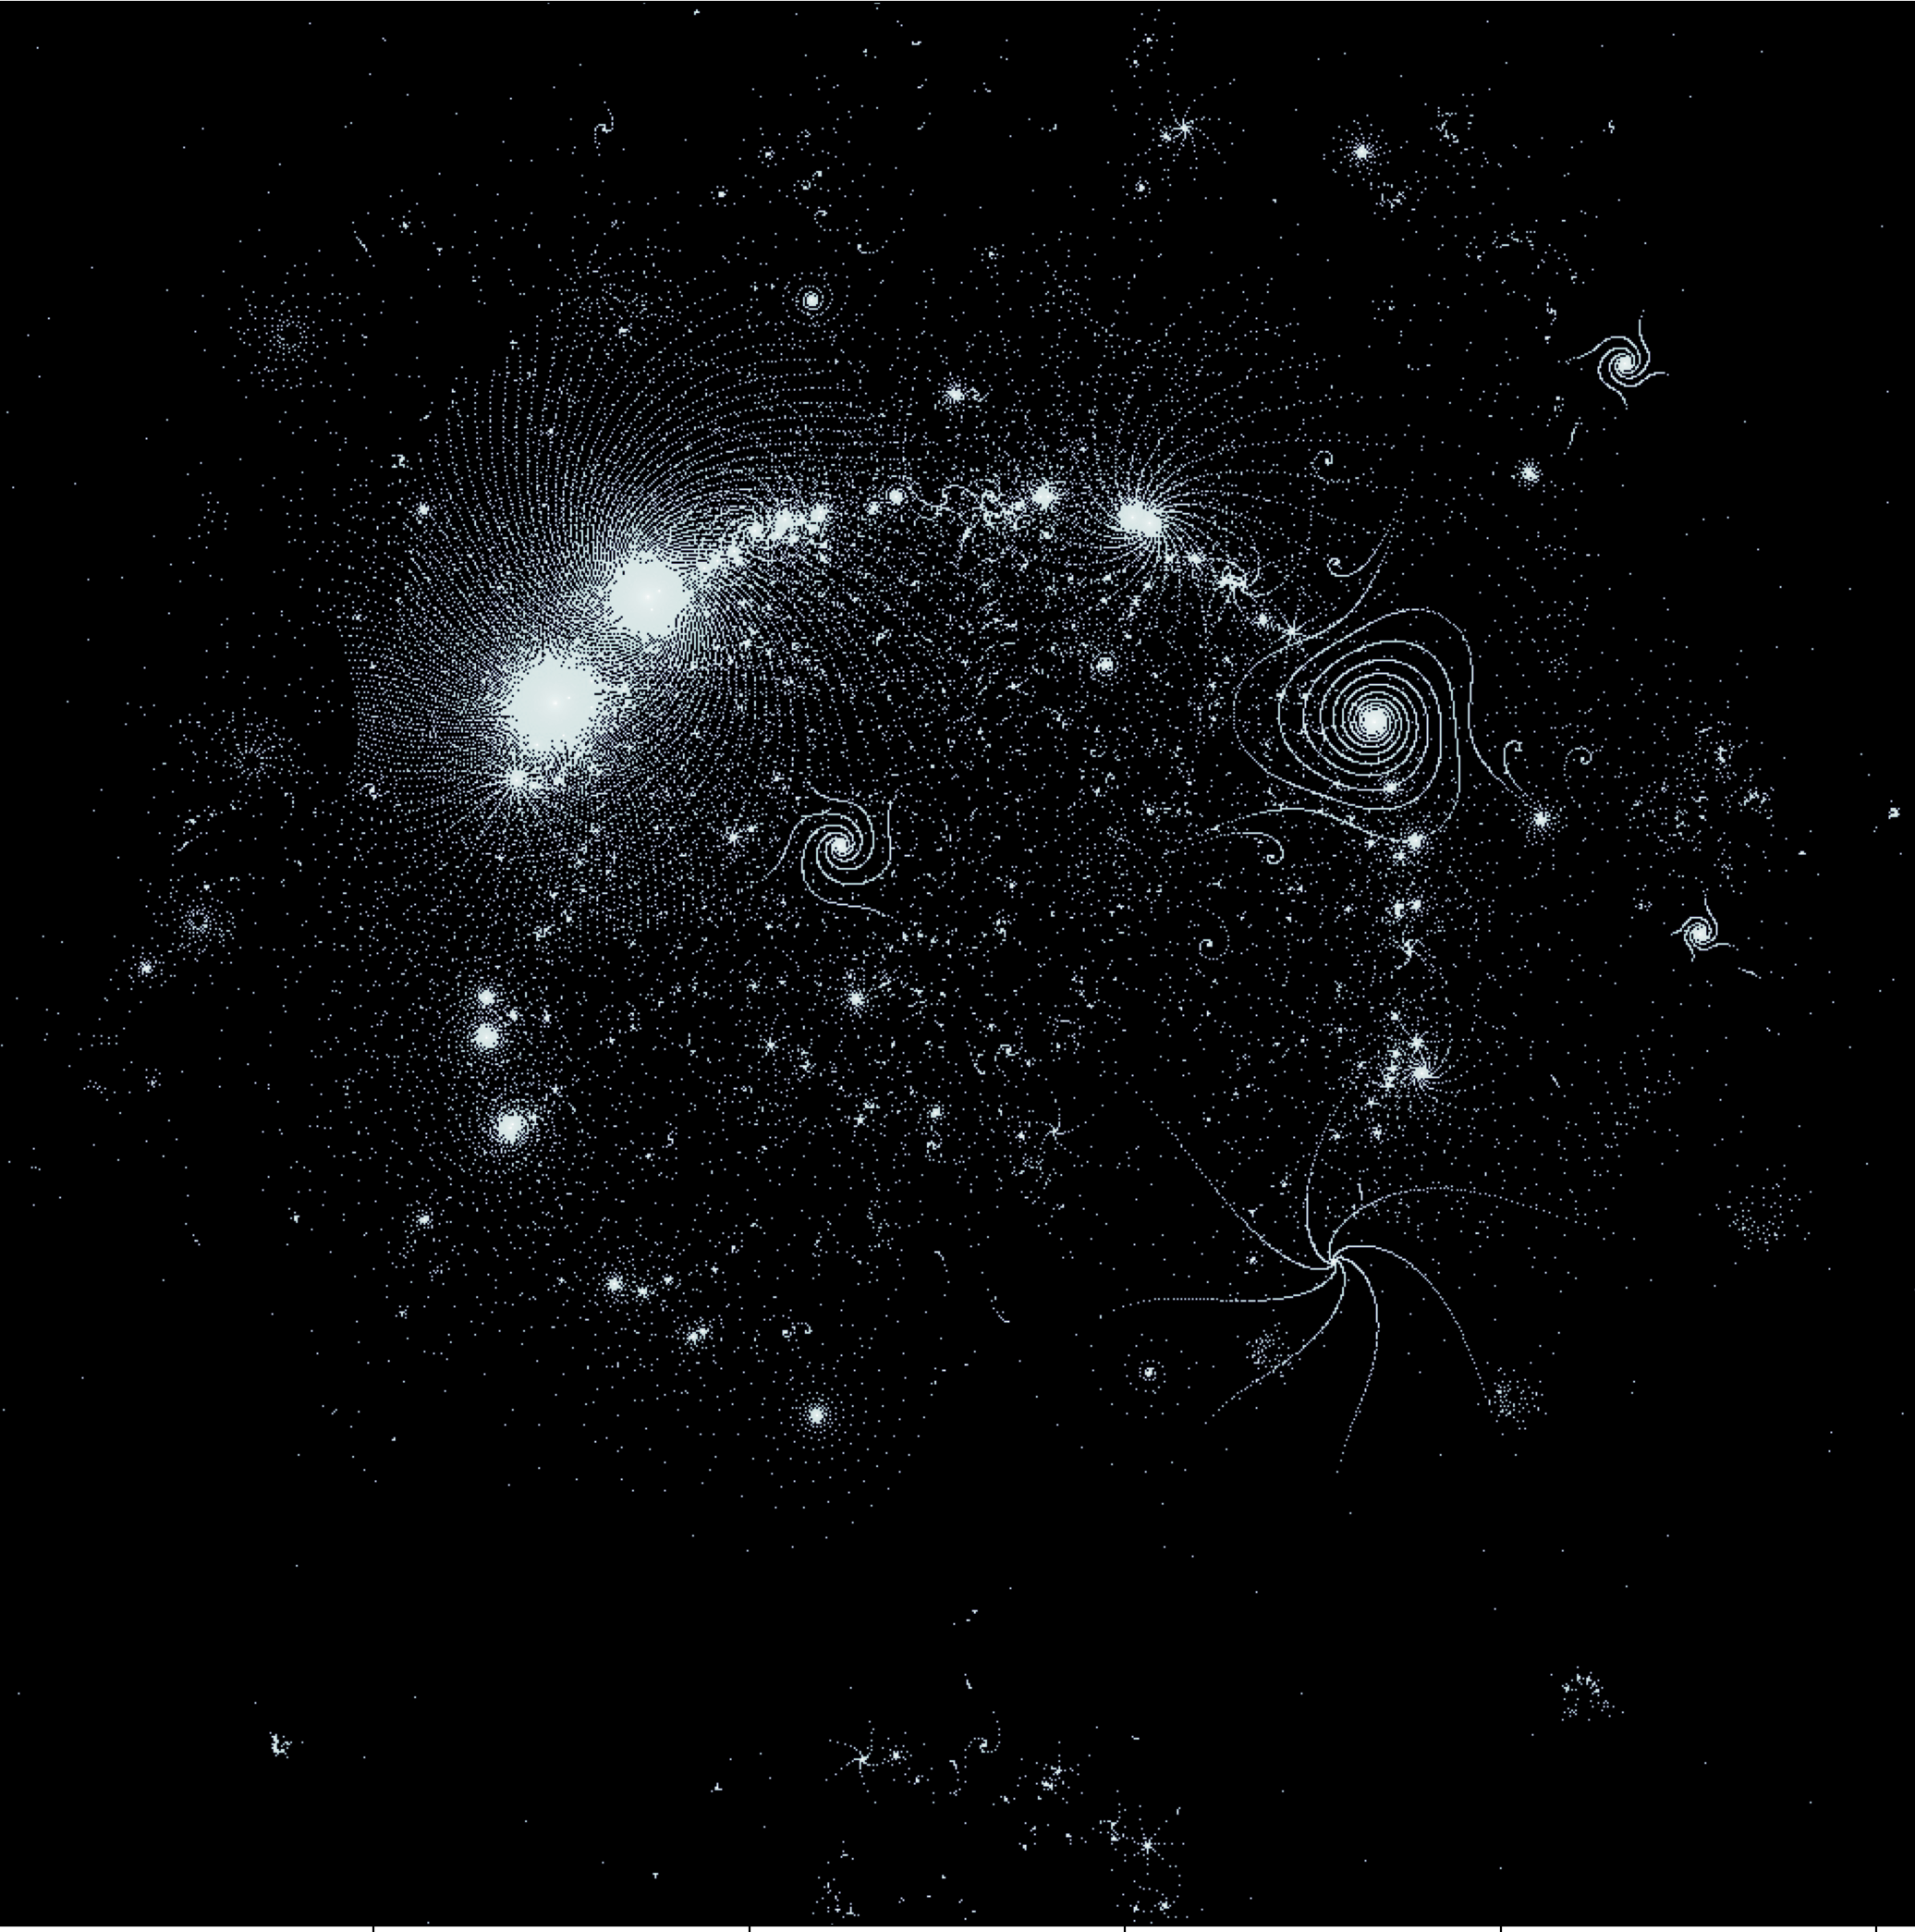
\includegraphics[width=0.55\textwidth]{code/buddhabrot.png}
    \end{center}
    \codecaption{code/buddhabrot.py}{Sp"at divergierende Orbits der Mandelbrot-Iteration.}\label{py:buddhabrot}
\end{listing}

Um zu sehen, wie Systeme von ihrem Anfangszustand abh"angen k"onnen, wollen hierf"ur ein etwas einfacheres Beispiel betrachten. 
Gegeben ist das System
\[
y[n] = \Sum{k=-\infty}{n}{x[k]}.
\]
Wir sehen hier, dass es f"ur die Berechnung von $y[n]$ nicht ausreicht, den Zustand des Eingangs zum Zeitpunkt $n$, also $x[n]$ zu kennen.
Schlie"slich m"ussen wir die gesamte Vergangenheit von $x[\cdot]$ bis zum Zeitpunkt $n$ in die Berechnung einflie"sen lassen.
Wir k"onnen das System aber umschreiben in 
\[
y[n] = \Sum{k=-\infty}{n-1}{x[k]} + x[n] = y[n-1] + x[n],
\]
wobei wir nun auch sehen, warum dieses System \emph{Akkumulator} genannt wird, da $y[\cdot]$ im Prinzip die Werte von $x[\cdot]$ \q{aufsammelt}.

Stellen wir uns nun vor, dass wir dieses System modellieren/simulieren wollen f"ur $n \leqslant n_0$, so ben"otigen wir entweder die Werte $x[n]$ f"ur $n < n_0$, oder die sogenannte \emph{Anfangsbedingung} $y[n_0] = y_0$.
Dies erinnert an das L"osen einer Differentialgleichung
\[
\dot{y}(t) = x(t),
\]
wonach dann gilt, dass
\[
y(t) = \Int{-\infty}{t}{x(s)}{s} 
\Text{oder}
y(t) = y_0 + \Int{t_0}{t}{x(s)}{s},
\]
damit $y(t_0) = y_0$.
Ein Beispiel f"ur die Wirkung von einem Akkumulator ist in \Cref{py:accumulator} gegeben. 
Man sieht sehr gut, welchen Einfluss die Anfangsbedingung auf $x_2[\cdot]$ hat, da dies den Grenzwert $\lim_{n \rightarrow \infty} y[n]$ ma"sgeblich beeinflusst.
Falls gilt, dass $y_0 = 0$, so spricht man vom Ruhezustand, beziehungsweise dem Nullzustand in dem sich das System zum Zeitpunkt $n = n_0$ befindet.
%
\begin{listing}
    \noindent
    \begin{minipage}{0.49\textwidth}
        \strut\vspace*{-\baselineskip}\newline
        \inputminted[firstline=4,lastline=18]{python3}{code/accumulator.py}
    \end{minipage}%
    \begin{minipage}{0.49\textwidth}
        \strut\vspace*{-\baselineskip}\newline
        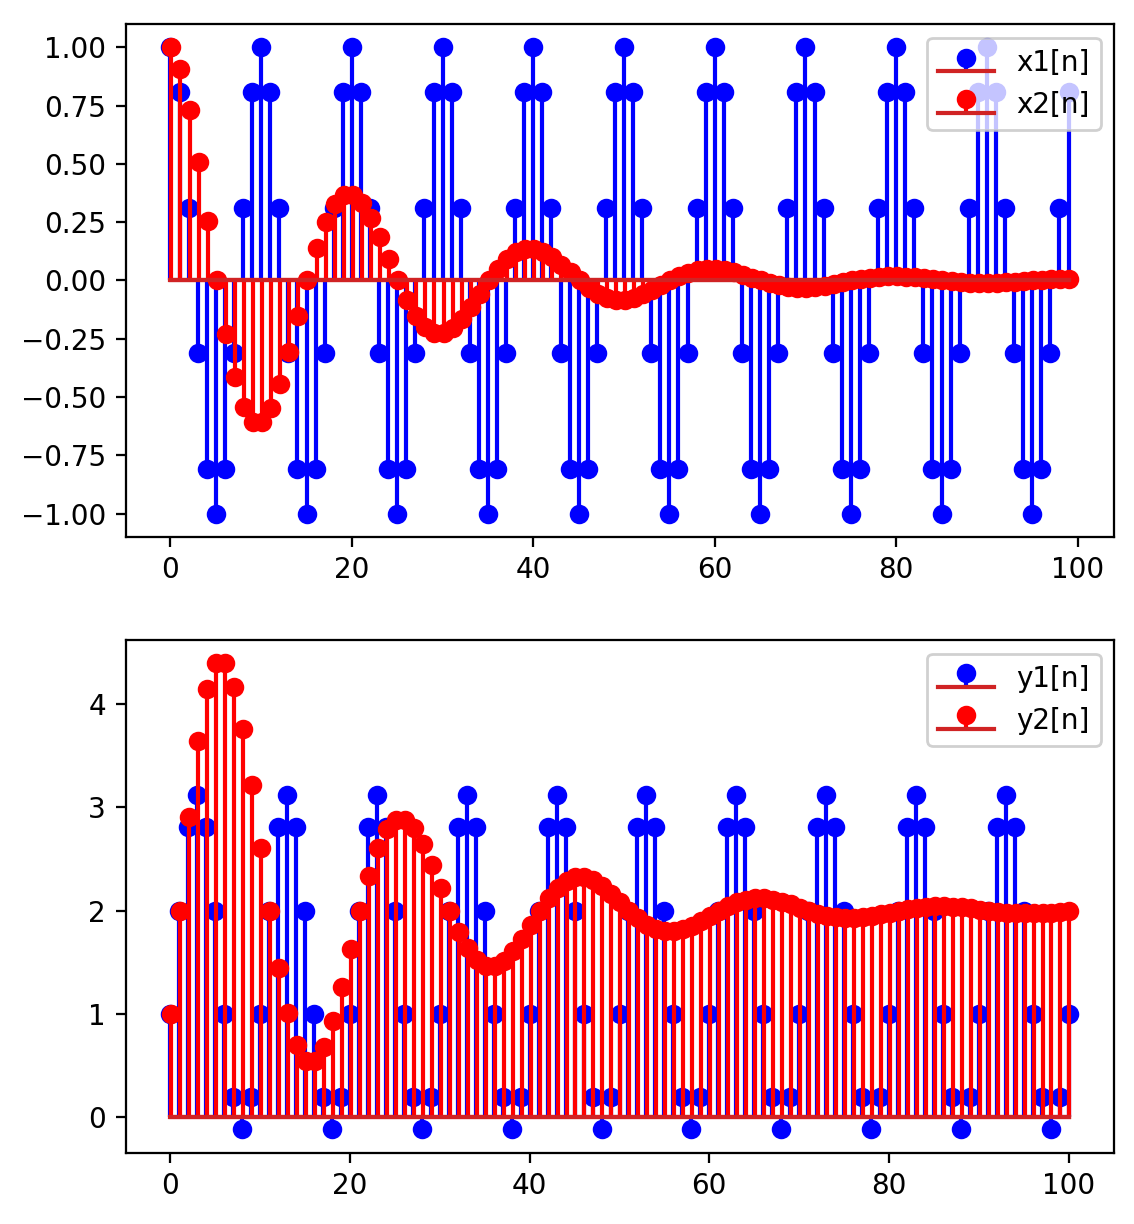
\includegraphics[width=\textwidth]{code/accumulator.png}
    \end{minipage}%
    \codecaption{code/accumulator.py}{Akkumulator f"ur zwei verschiedene Eingangsignale.}\label{py:accumulator}
\end{listing}

\paragraph{Statisch vs. Dynamisch}
Man kann Systeme nun auf verschiedene Arten klassifizieren.
Beispielsweise nennen wir Systeme \emph{statisch}, wenn der Wert $y[n]$ nur von $x[n]$ abh"angt, aber nicht von vergangenen oder gar zuk"unftigen Werten (entweder von $y[\cdot]$ oder $x[\cdot]$).
Die Systeme
\[
y[n] = a x[n], \Text{oder} y[n] = \sqrt{x[n]} + x^4[n]
\]
sind statisch.
H"angt nun $y[n]$ von seiner eigenen Vergangenheit oder der von $x[n]$ ab, so nennen wir diese Systeme dynamisch, oder Systeme mit Ged"achtnis.
Die Systeme
\[
y[n] = x[n] + a x[n-1] \Text{,} y[n] = \Sum{k=0}{N}{x[n-k]}
\]
sind dynamisch und haben jeweils Ged"achtnis der L"ange $g = 1$, beziehungsweise $g = N-1$.
Man sieht bereits an \Cref{py:accumulator}, dass dynamische System im Allgemeinen interessanter sein werden.

\paragraph{Kausal vs. Akausal} 
H"angen die Werte $y[n]$ nur von $x[n], x[n-1], \dots$ ab, also nicht auch von $x[n+1], x[n+1], \dots$, so nennen wir das System kausal.
Intuitiv bedeutet dies die intuitiv bekannte Kausalit"at in dem Sinne, dass nur die Zeitliche Vergangenheit notwendig ist, um den aktuellen Zustand des Systems zu bestimmen.
Ist die nicht gegeben, so nennt man das System \emph{akausal} oder \emph{nicht-kausal}.

Was die Realisierung von akausalen Systemen angeht, wird es nicht m"oglich sein, diese in Echtzeit umzusetzen, da man diese nur mit einer Verz"ogerung, oder gar nicht f"ur sequentiell verf"ugbares $x[\cdot]$ implementieren kann.
Sind die Werte $x[n]$ jedoch beispielsweise durch Messung oder Simulation entstanden und \q{offline} verf"ugbar, so k"onnen solche Systeme durchaus angewandt werden und n"utzlich sein.

\paragraph{Stabil vs. Instabil} Eine der zentralen Eigenschaften, die auch bei analogen Systemen eine Rolle spielt ist Stabilit"at.
Zwar hat man normalerweise bereits einen intuitiven Begriff f"ur Stabilit"t im Sinn, doch formal gibt es hiervon verschiedene Auspr"agungen.
Wir beschr"anken uns auf die Version der \gls{bibo}-Stabilit"at, welche fordert, dass f"ur beschr"anktes Eingangssignal $x[\cdot]$ der Ausgang $y[\cdot]$ ebenfalls beschr"ankt bleibt.
Formal fordern wir also, dass falls
\[
\Abs{x[n]} \leqslant M_x \Text{f"ur alle} n \in \Z
\]
f"ur eine Konstante $M_x \in \R$ gilt, dann auch 
\[
\Abs{y[n]} \leqslant M_y \Text{f"ur alle} n \in \Z
\]
gelten muss. 
Man sieht, dass $M_x$ und $M_y$ an $x[\cdot]$ und $y[\cdot]$ gebunden sind, also keine \q{universellen} Konstanten sind.
Andersherum reicht es also f"ur Instabilt"at nur \emph{ein} beschr"anktes Eingangssignal $x[\cdot]$ konstruiert werden muss, f"ur welches $y[\cdot]$ nicht beschr"ankt bleibt.
Betrachten wir folgendes
\begin{Exm}
Gegeben sei
\[
y[n] = C \cdot y[n-1]^2 + x[n]
\]
und wir nutzen als Eingang den Einheitssto"s $x[\cdot] = C \delta[\cdot]$, welcher beschr"ankt ist, mit $M_x = \Abs{C}$ f"ur $C \in \R$.
Doch dieser produziert f"ur $y[n] = 0$ f"ur $n \leqslant -1$ die Folge
\[
y[n] = \{0, \Start{C}, C^2, C^4, \dots, C^{2n}\},
\]
welche f"ur $\Abs{C} > 1$ gegen $\infty$ divergiert.
\end{Exm}

\paragraph{Zeitvariant vs. Zeitinvariant} Systeme deren Eingabe-Ausgabe-Verhalten nicht zeitlich konstant ist, nennt man \emph{zeitvariant}.
Systeme, die f"ur zeit verz"ogerte Eingaben, die um den gleichen Zeitraum verz"ogerte Ausgaben produzieren, nennt man \emph{zeitinvariant}, siehe \Cref{exm:cont_lit}.
Formal fordern wir f"ur Zeitinvarianz, dass wenn f"ur beliebige Eingabe $x[\cdot]$
\[
x[\cdot] \overset{\mathcal{T}}{\rightarrow} y[\cdot]
\]
gilt, dass dann f"ur jedes $k \in Z$ auch gilt, dass
\[
x[\cdot -k] \overset{\mathcal{T}}{\rightarrow} y[\cdot - k]
\]
erf"ullt ist.
In der Schreibweise von \eqref{eq:gen_disc_sys} hei"st dies, dass f"ur 
\[
    y[n] = \mathcal{T}(x[\cdot])[n]
\]
auch gelten muss, dass
\[
    y[n - k] = \mathcal{T}(x[\cdot - k])[n]
\]
und zwar f"ur alle $x[\cdot]$ und $k$.

Was erst einmal relativ abstrakt daherkommt, ist eigentlich eine sehr intuitive Sache. 
Wenn wir beispielsweise an ein Audiointerface denken, so h"atten wir schon gerne, dass es egal ist, zu welchem Zeitpunkt jemand ins Mikrophon singt -- unabh"angig vom Zeitpunkt sollte die Aufnahme \q{gleich klingen}.
Das System, welches die Aufnahme und eventuelle Audioverarbeitung realisiert, sollte keine zeitlichen Ver"anderungen zeigen.
Auch in der umgekehrten Richtung, beim Abspielen von Ton, sollte es irrelevant sein, zu welchem Zeitpunkt man ein gewisses St"uck h"oren m"ochte -- das H"orerlebnis sollte davon nicht beeinflusst sein.

Im Grunde ist Zeitinvarianz also etwas, das wir normalerweise von einem System \q{erwarten} und nicht untersuchen wollen.

\paragraph{Linear vs. Nicht-Linear} Kommen wir zum Schluss dieser Klassifikationen zu einer der wichtigsten Unterscheidungen.
Ein System, das f"ur Eing"ange $x_1[\cdot]$ und $x_2[\cdot]$ die Antworten
\[
    y_1[n] = \mathcal{T}(x_1[\cdot])[n]
    \Text{und}
    y_2[n] = \mathcal{T}(x_2[\cdot])[n]
\]
produziert, nennen wir \emph{linear}, falls die Antwort des Systems auf den Eingang
\[
    x[\cdot] = a_1 x_1[\cdot] + a_2 x_2[\cdot]
\]
sich durch
\[
    y[n]
        = \mathcal{T}(x[\cdot])[n] 
        = \mathcal{T}(a_1 x_1[\cdot] + a_2 x_2[\cdot])[n] 
        = a_1 \mathcal{T}(x_1[\cdot])[n] 
            + a_2 \mathcal{T}(x_2[\cdot])[n] 
\]
ausdr"ucken l"asst.
%
\begin{figure}
    \centering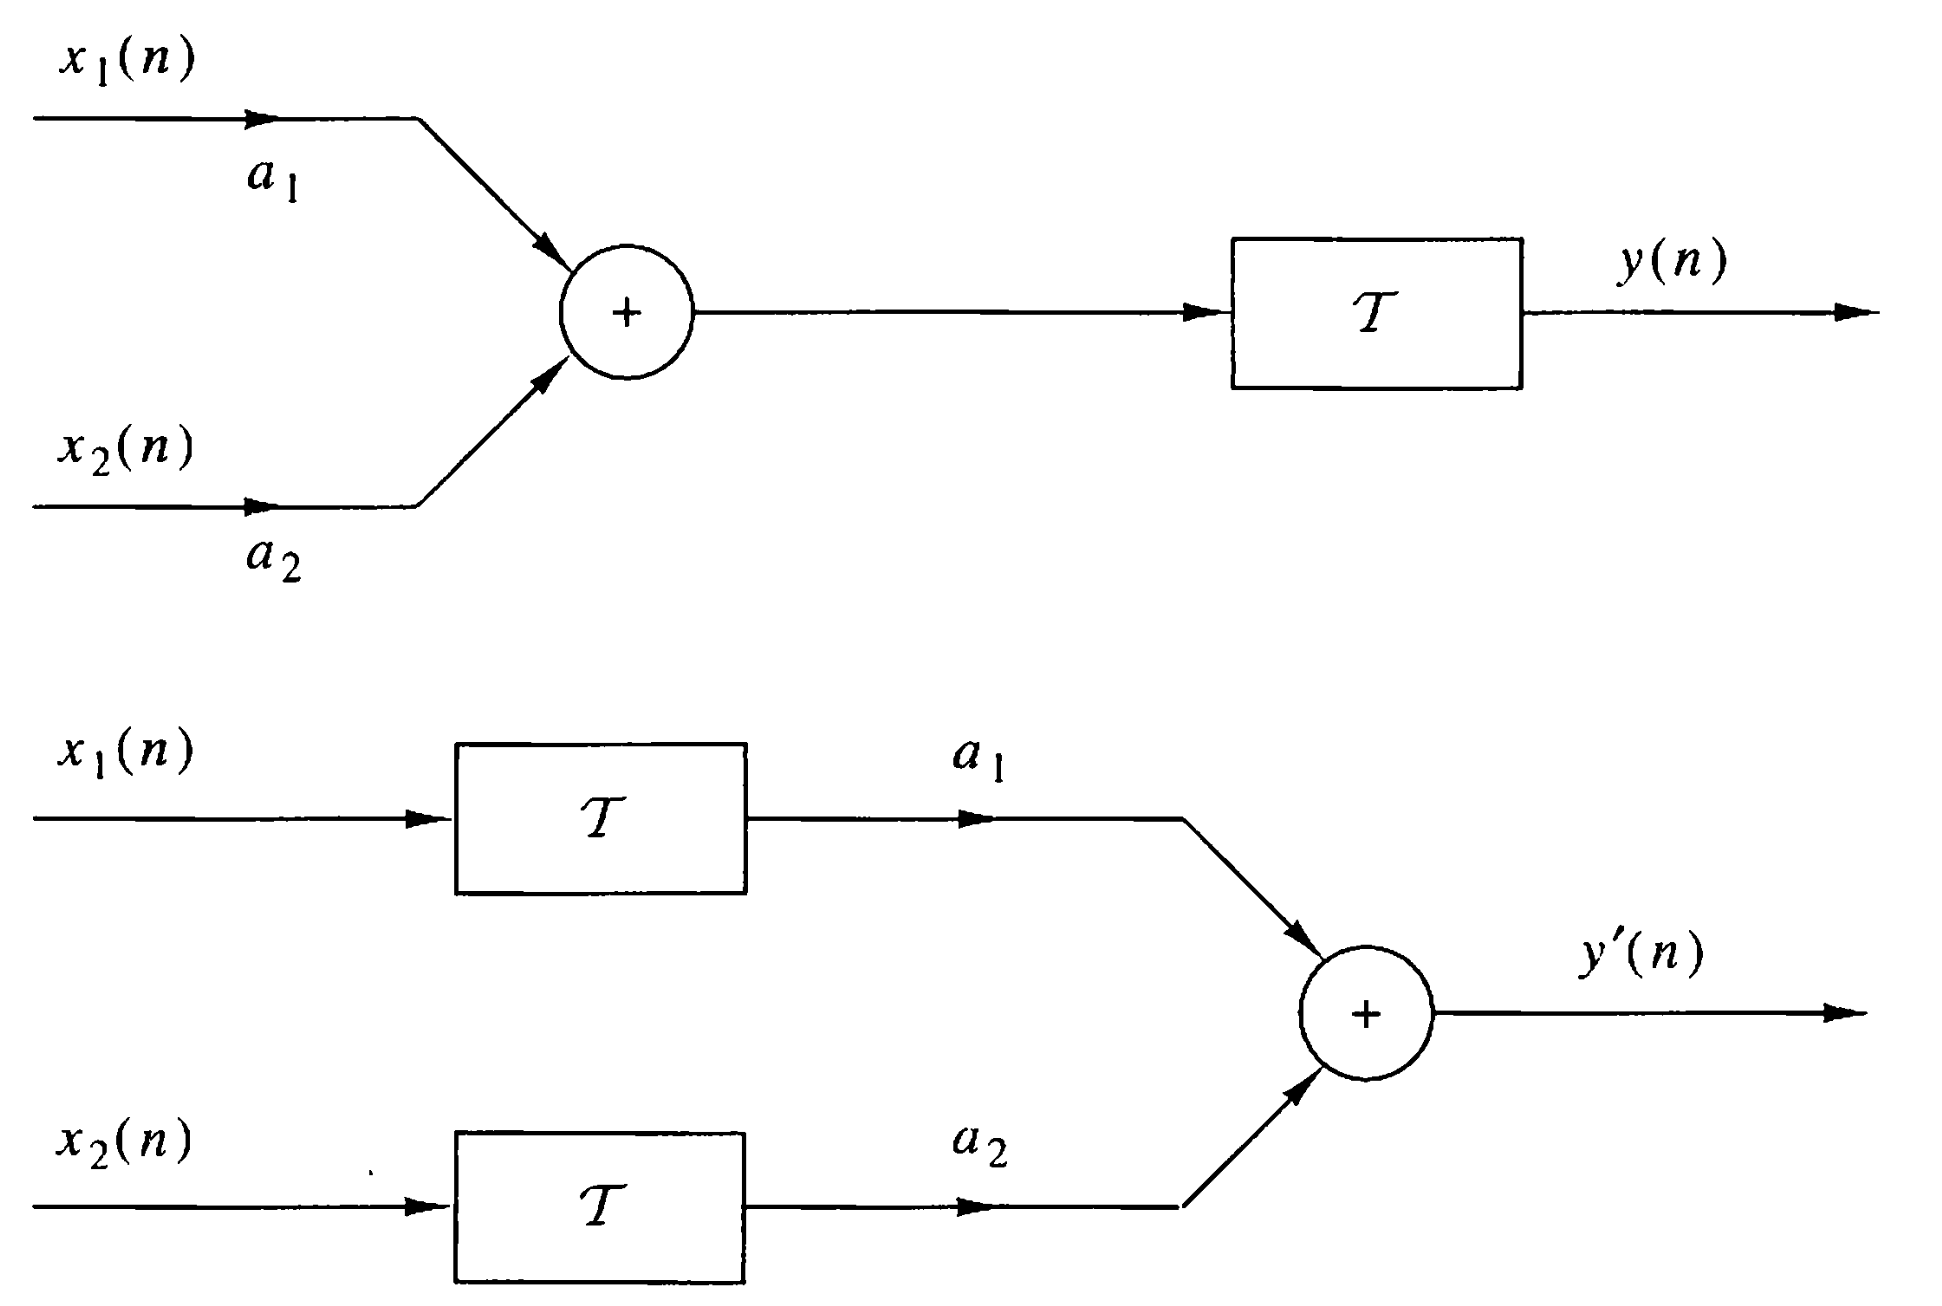
\includegraphics[width=0.6\textwidth]{img/disc_sys/linear_sys.png}
    \caption{zeigt zwei verschiedene systemtheoretische Interpretation von linearen Systemen. Quelle: \cite{proakis2013}}\label{img:disc_sys:linear_sys}
\end{figure}
%

\Cref{img:disc_sys:linear_sys} zeigt die beiden m"oglichen Interpretationen dieser Eigenschaft.
Man kann sich also vorstellen, dass die Eing"ange \emph{erst} skaliert und addiert werden und dann das System durchlaufen, oder man prozessiert beide Eing"ange durch $\mathcal{T}$ und skaliert und addiert die \emph{Ausg"ange nachdem} das System im Grund \q{zweifach} angewandt wurde.

Anders gesagt \q{passen} lineare Systeme genau zu der linearen Struktur von Signalen, wenn wir sie als Vektoren in einem Vektorraum auffassen.
Als Konsequenz ergibt sich, dass sich lineare Systeme deutlich einfacher analysieren lassen, weil wir Werkzeuge der linearen Algebra benutzen k"onnen.
Diese Eigenschaft ist so attraktiv, dass man oft versucht nichtlineare Systeme durch geeignete lineare System zu approximieren (Bsp: Pendel $\sin(x) \approx x$).
Man nimmt also Fehler in der Analyse in Kauf, ist damit aber immerhin in der Lage "uberhaupt Aussagen treffen zu k"onnen.
%
\subsubsection{Diskrete \texorpdfstring{\acrshort{lti}}{LTI} Systeme}\label{sec:disc_sys:disc_lti}
Wir schr"anken nun die Menge der Systeme ein, die wir betrachten wollen, indem wir fordern, dass das System $\mathcal{T}$ gleichzeitig linear und zeitinvariant ist.
\begin{itemize}
    \item wiederholung der eigenschaften: shift-invarianz, linearitaet
    \item reaktion auf signal, das aus bausteinsignalen zusammengesetzt wurde
    \item darstellung als summe von skalierten, geshifteten einheitsstoessen
    \item faltungsformel
    \item algorithmus zur berechnung
    \item exerzieren von beispiel 2.3.2, uebung programmieren (naiv summieren, scipy convolve)
    \item exerzieren von beispiel 2.3.3, uebung programmieren der approximation
    \item assoziativitaet, kommmutativitaet
    \item cascadierung von mehreren systemen
    \item stabilitaet: $h[n]$ muss absolut summierbar sein, gegen $0$ gehen
    \item beispiel 2.3.6. (fuer uebung irgendwas ausdenken)
\end{itemize}

\subsubsection{Cross- und Autokorrelation}\label{corr}

\begin{itemize}
    \item Definition
    \item eigenschaften
    \item synthetisches beispiel schwingung + noise, akf zeigt periodizitaet
    \item beispiel mit woelfer sunspot numbers
    \item beispiel mit m-sequenzen, niklas einladen, schaltung zeigen
    \item monster uebung: 2.65
\end{itemize}